\section{Structure}\label{sc:structure}
% Intro intro
Based on the analysis in the former sections, the structure of the classes in the problem domain has been visualised in a class diagram (see \autoref{fig:FirstPDClassDiagram}).

\begin{figure}[H]
    \centering
    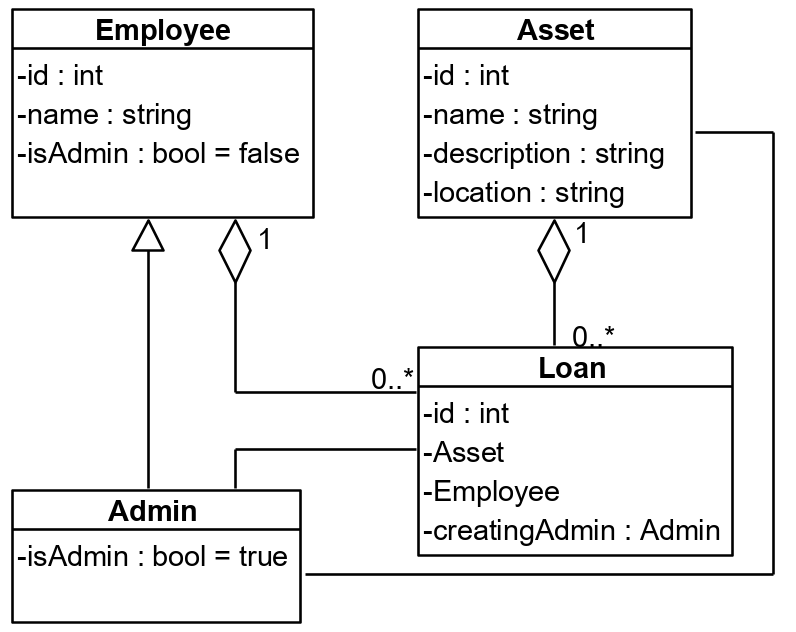
\includegraphics[width=0.8\textwidth]{figures/PDDiagramV6.png}
    \caption{Class diagram of the classes in the problem domain.}
    \label{fig:FirstPDClassDiagram}
\end{figure}

As described in \autoref{sc:classes}, there are four different relevant classes in the problem domain. These classes are: \textbf{Employee}, \textbf{Admin}, \textbf{Asset}, and \textbf{Loan}. The relations between these have been explained below.
\newline

The \textit{Employee} class is a super class, as it does not aggregate from or specialize any other classes.
\newline

The \textit{Asset} class is also a super class as it does not aggregate from or specialize another class. The \textit{Asset} associates with the \textit{Admin} class as the \textit{Asset} stores which \textit{Admin} modified or created it.
\newline

The \textit{Admin} class is a specialization of the \textit{Employee} class, as the \textit{Admin} class contains the same information as the \textit{Employee} class, but the \textit{isAdmin} attribute is true, which give this class access to more functionality in the system. The \textit{Admin} class also contains associations to assets and loans, because an admin in the system can create and modify assets and loans.
\newline

The \textit{Loan} class is created to handle the relation between the \textit{Asset} and \textit{Employee} classes. The \textit{Loan} class aggregates from the \textit{Employee} class, because an employee can be in possession of multiple assets, and therefore have multiple active loans. It aggregates from the \textit{Asset} class, as the asset contains a history of previous loans. The involved asset, employees, and creating admin are stored on the \textit{Loan} class upon creation.
\newline
\par

With the classes of the problem domain and their relations to each other described, their behaviour can be examined.